\chapter{Revisão Bibliográfica}
%% Visão geral sobre carregadores de veículos elétricos.

\cite{Baharom:2024} comentam sobre futuros avanços tecnológicos no carregamento de veículos elétricos. O texto aborda especificamente sobre os desafios de desenvolver um carregador onboard bidirecional, que incluem a dificuldade de gerenciar o fluxo de potência em ambos os sentidos, a complexidade necessária para o sistema de controle e a integração desses sistemas com a rede elétrica existente. Ademais, o artigo aborda sobre o carregamento indutivo sem fio e justifica a necessidade em pesquisa nessa tecnologia com base na maior segurança e menor necessidade de manutenção obtida. Ao mesmo tempo, os autores reconhecem que a limitação na transferência de potência sem fios e a baixa eficiência inviabilizam esse sistema na prática.

De acordo com \cite{Kumar:2021}, os convesores CA-CC bidirecionais, que estão presentes em carregadores de carros elétricos, apresentam desafios em
relação a sincronização de frequência e fase, controle do fator de potência e qualidade de
isolação.

%% Visão sobre o PFC.

Os \textit{application notes} \cite{onsemi_hbd853} e \cite{ti_zhcp224} apresentam uma visão
geral sobre o controle do fator de potência ativo com um conversor boost monofásico. Esse
conversor pode operar tanto em modo de condução contínua (CCM) quanto em modo de condução
crítica (CRM). Em CCM, o conversor é controlado através do controle pelo modo de corrente
média. Nesse cenário, a malha de controle externa é lenta e tem o papel de ajustar o valor de
tensão de saída enquanto que a malha de controle de corrente(interna) é mais rápida e visa
fazer com que a corrente média do indutor siga a forma de onda de uma entrada de referência
senoidal que esteja em fase com a tensão da rede. Já a operação em CRM é adequada apenas para
uma potência de saída abaixo de 300 W e caracteriza-se pelo controle através de um sinal PWM
com frequência de cheaveamento variável e tempo ON constante.

Em relação ao retificador PFC trifásico, tanto \cite{3phPlecs} quanto \cite{WANG2013/03}
realizam o controle do conversor CA-CC por meio da transformada de Park. Nessa metodologia, um
\textit{Phase Locked Loop} (PLL) captura a referência de fase da tensão de entrada, que em
seguida é utilizada na transformação para o sistema de coordenadas dq0.Ademais, duas malhas de
controle, uma externa, referente à tensão de saída do retificador e uma interna, que controla
as componentes de eixo direto e em quadratura da corrente de entrada. Como o objetivo é
controlar o fator de potência, a componente de corrente em quadratura é ajustada para ser nula.

O artigo da ONSEMI \cite{} aborda as principais topologias de retificadores PFC trifásicos. A primeira topologia citada é o retificador PWM Vienna (Fig.), que é caracteriado como uma de ponte retificadora trifásica conectada a uma conversor boost por fase. A topologia Vienna tem como principal vantagem o uso de apenas um transistor por fase, o que simplica significativamente o controle do conversor e o cheaveamento em três níveis, ao mesmo tempo, o alto número de diodos nessa topologia implica em maiores perdas. Já topologia T-NPC é derivada da Vienna e consiste basicamente numa ponte de diodos trifásica conectada a seis transistores. A principal vantagem dessa topologia é o menor número de componentes em relação à anterior. Ambas as topologias citadas são unidirecionais. Ademais, a topologia T-NPC pode ser implementada apenas com transistores, o que a torna bidirecional.

\begin{figure}[h]
	\centering
	\begin{minipage}{0.45\textwidth}
		\centering
		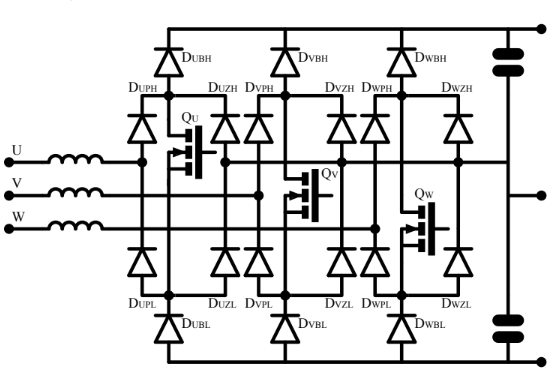
\includegraphics[width=\textwidth]{./Figuras/PFC_Vienna.png}
		\caption{Retificador PFC Vienna.}
		\label{fig:pfc_vienna}
	\end{minipage}
	\hfill
	\begin{minipage}{0.45\textwidth}
		\centering
		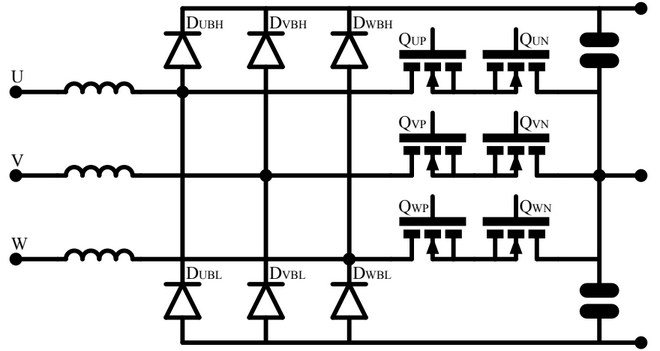
\includegraphics[width=\textwidth]{./Figuras/PFC_TNPC.png}
		\caption{Retificador T-NPC.}
		\label{fig:pfc_tnpc}
	\end{minipage}
\end{figure}

A principal topologia de retificador PFC trifásico é a \textit{Six-switch rectifier}, que consiste numa ponte trifásica formada por seis transistores de tensão nominal na faixa de 900 V a 1200 V. A principal vantagem dessa topologia é a bidirecionalidade, inclusive porque o inversor trifásico a seis transistores é frequentemente utilizado no acionamento de motores elétricos. Ao mesmo tempo, esse retificador apresenta maior interferência eletromagnética que as outras opções citadas.

Conforme a figura \ref{fig:controlepfc3ph}, o controle do PFC trifásico

\begin{figure}
	\centering
	\caption{Esquema de controle do PFC trifásico.}
	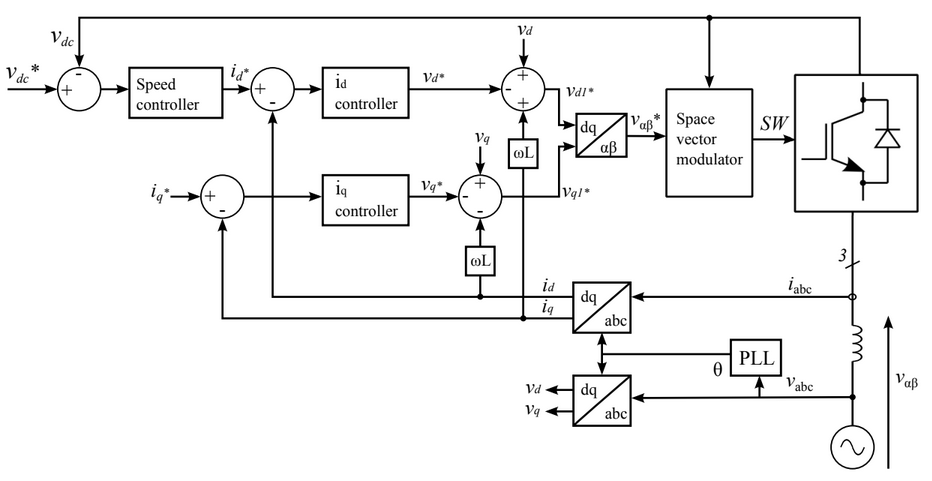
\includegraphics[width=0.8\textwidth]{./Figuras/controlepfc3ph.png}
	\legend{Fonte: \cite{3phPlecs}.}
	\label{fig:controlepfc3ph}
\end{figure}